\section{Methodology}

This section covers the details of technical solutions used in the project and
aims to provide an understanding of why certain decisions were made, certain
tools and technologies were used.

\subsection{High Level Overview}

From a high level perspective CodeGlass consists of three main components:

\begin{itemize}
    \item Browser Extension (front-end)
    \item Application Server (back-end)
    \item LLM (AI) Adapter
\end{itemize}

Their composition can be inspected on the following figure.

\begin{figure}[h]
    \centering
    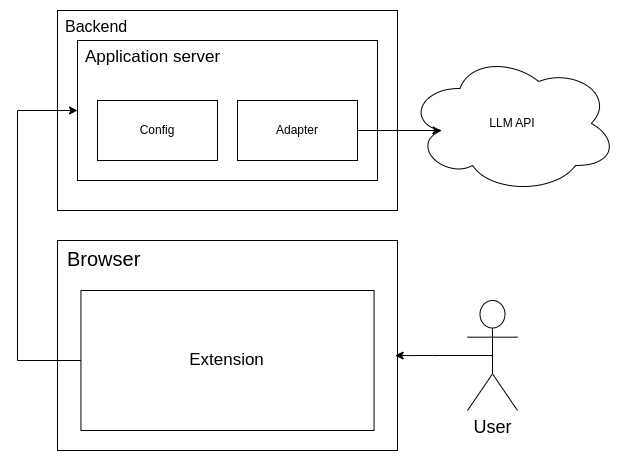
\includegraphics[width=0.9\textwidth]{assets/hl-arch.png}
    \caption{This is an example image}
    \label{fig:hl}
\end{figure}

The main idea behind using separate component for back-end, instead of realizing
the interactions directly between the \emph{Extension} and \emph{LLM API}, is to
provide an easy way for user to extend the tool and modify it to suit their needs,
without need to extend and/or modify the \emph{Extension}, as browser extension
development introduces specific challenges. As an addition keeping sensitive data
(such as API keys) in the browser introduces additional implications related to
security.

The project also aims to allow users to self-host the whole setup in order to avoid
potential trust issues.

Due to the time-pressure all components were implemented in plain JavaScript,
without Typescript usage.

\subsection{Extension}

Extension component is responsible for tracking user's text highlighting events.
It consists of content script, background worker and popup window.

This text highlighting event capturing mechanism is realized in the content script
using "mouseup" DOM \autocite{DOM} event and window.getSelection method.

Once the event is captured event listener checks if user selection is not empty, if
so sends an internal message via chrome.runtime.sendMessage method to the background 
worker.

On receiving highlighted text Background worker sends two sequential HTTP
\autocite{HTTP} requests to the \emph{Application Server}. First one to the
`/isCode` endpoint to the application server to use LLM for determining if the
highlighted text is some kind of programming code or markup language that should be
analyzed. If server return `false` here the pipeline stops, otherwise the second
request is sent to obtain structured analysis summary payload, that extension
can render on the page inside the popover element.

The extension's source code is structured in the following way:
\begin{itemize}
    \item `api` directory hold all the functions and constants needed to
        communicate with the \emph{Application Server}.
    \item `content` directory holds the main content script code.
    \item `css` directory holds CSS styles files.
    \item `pages` directory holds HTML file for extension's pop-up page.
    \item `popover` directory holds functions and constants related to rendering
        popover element.
    \item `storage` directory holds function and constants needed for storing and
        retrieving values from chrome.storage.local.

    \item `background.js` is sort of an entry point for the background worker.
    \item `popup.js` file is a script for pop-up page.
    \item `manifest.json` is a main manifest file which defines the extension's
        metadata, permissions, scripts, and behaviors, serving as the central
        configuration for how the extension interacts with the browser.
\end{itemize}

\subsection{Application Server}

\subsection{Adapter}

